\chapter{Einleitung}
In diesem Kapitel werden die relevanten Konzepte des Schienengüterverkehrs im Zusammenhang mit unserer Problemstellung vorgestellt, wobei nach einer kurzen Einführung die Hintergrundauskünfte und Terminologie im Unterabschnitt \hyperref[sec:problem]{1.1.1} erklärt werden. Es folgt eine ausführliche Problemdarstellung im Unterabschnitt \hyperref[sec:discription]{1.1.2} , und eine Zusammenfassung des aktuellen Lösungsansatzes im Unterabschnitt \hyperref[sec:current]{1.1.3}.\\
Schließlich wird im Abschnitt \hyperref[sec:Ziel]{1.1.2} das Ziel dieser Abschlussarbeit bezüglich der beschriebenen Problematik im vorherigen Abschnitt verdeutlicht.

\section{Problematik}
\label{sec:problem}
In langfristiger Hinsicht nimmt Güterverkehr bei globalisierten Märkten zu, und Deutschland als zentrale Verkehrsverbindung spielt eine wichtige Rolle in Logistik von Europa. DB Cargo ist ein führender globaler Logistikdienstleister und der größte Anbieter im Schienengüterverkehr in Europa. Schienenverkehr ist eine ökonomische und umweltfreundliche Form der Transportation. Es dient zur Verteilung der sowohl schweren Container wie Massengüter von Kohlen oder Stahl als auch kleineren Sendungen, die nur einen Teil des gesamten Zugs besetzen. Entwurf eines Verwaltungssystems zur Fahrplanung und Konsolidierung der Sendungen unter minimierten Kosten ist jedoch eine große Herausforderung.

\todo{absprechen} DB Schenker ist ein führender globaler Anbieter der Logistikdienstleistungen, der weltweit Industrie und Handel beim Güteraustausch durch Landverkehr, Luft- und Seefracht, Kontraktlogistik und Supply Chain Management unterstützt. Mit 430 Standorten für den europaweiten Landverkehr ermöglicht DB Schenker Güterströme zwischen beiden Verkehrsträgern (bzw. auf der Straße oder Schiene) in einem umfassenden Netzwerk. Damit verbindet er die besonderen Vorteile der einzelnen Transportarten durch innovative multimodale Lösungen, um die Sendungen termingerecht mit höherer Flexibilität zu transportieren. Entwurf eines Verwaltungssystems zur Fahrplanung und Konsolidierung der Sendungen unter minimierten Kosten ist jedoch eine große Herausforderung.

\subsection{Problemspezifische Begriffe und Parameter}
Um die Problemdarstellung besser nachzuvollziehen und die Parameter des Modells kennenzulernen, wird im folgenden Unterabschnitt die notwendige technische Terminologie aus dem Güterverkehrssystem sowie deren Parameter dargestellt.

\subsubsection{Wagen}
Ein Wagen ist eine meist vierrädrige Ladeeinheit zum Beladen der Güter und bezeichnet die kleinste Transporteinheit. Er verfügt üblicherweise über keinen Antrieb, deswegen wird eine Kupplung der Wagen mit einer Lokomotive gezogen. Es gibt verschiedene Arten von Güterwagen, die je nach Güterformen spezifiziert worden sind. Bei dieser Arbeit wurden die Wagen jeder Sendung als gleich angenommen. Die Wagen verschiedener Sendungen können jedoch unterschiedliche Kosten verursachen.

\subsubsection{Anlagen (Bahnhöfe)}
Eine Anlage in Bezug auf Schienengüterverkehr ist eine Station (ein Bahnhof), wo die Güter ein- bzw. ausgeladen oder die Wagen zur Erstellung eines neuen Zugs umrangiert werden.\\
Folgende Tabelle zeigt die Parameter, die eine Anlage kennzeichnen.

\begin{table}[ht]
\centering
\begin{tabular}{lll}
\hline
\rowcolor[HTML]{000000} 
{\color[HTML]{FFFFFF} } & {\color[HTML]{FFFFFF} \textbf{Beschreibung}}                                           & {\color[HTML]{FFFFFF} \textbf{Parameter}} \\ \hline
\textbf{1}                   & \begin{tabular}[c]{@{}l@{}}Max. Anzahl der Wagen, die in Anlage $i$ umgestellt\\ werden \end{tabular}                           & MaxWagonCount          \\ 
\hline
\multirow{2}{*}{\textbf{2} } & \multirow{2}{*}{Max. Anzahl der ein- bzw. ausgehenden Züge an Anlage $i$}                                                       & MaxIngoingTrainCount   \\
                             &                                                                                                                               & MaxOutgoingTrainCount  \\ 
\hline
\multirow{2}{*}{\textbf{3} } & \multirow{2}{*}{\begin{tabular}[c]{@{}l@{}}Max. Anzahl der ein- bzw. ausgehenden Richtungsgleise\\ an Anlage $i$ \end{tabular}} & MaxOutgoingTrackCount  \\
                             &                                                                                                                               & MaxIngoingTrackCount   \\ 
\hline
\textbf{4}                   & Die Fixkosten der Anlage $i$                                                                                                   & FixedCosts             \\ 
\hline
\textbf{5}                   & Umstellkosten der Anlage $i$                                                                                                    & SwithCosts            \\
\hline
\textbf{6}                   & Die kosten der ausgehendenRichtungsgeleise der Anlage $i$                                                                                                    & OutgoingTrackCosts 
\end{tabular}
\caption{Liste der Parameter einer Anlage}
\end{table}

Die Kosten einer Anlage sind im Fall der Umstellung relevant, und bestehen aus drei Kostenkomponenten, nämlich den Fixkosten der Anlage, den Kosten der ausgehenden Richtungsgeleise und den Umstellkosten. Die Anlagenfixkosten verursachen einen Pauschalwert, falls die Anlage mindestens einmal in einer Sendungsroute vorkommt. Die Umstellkosten sind jedoch linear pro Sendungseinheit zu berechnen.

\subsubsection{Kanten}
Eine Kante verbindet zwei Anlagen und kann einer Sendungsmenge oder den Wagen zugeordnet werden. Die einer Kante zugeordneten Wagen fahren zu einer gewissen Abfahrtszeit gemeinsam  zum Endknoten der Kante, ohne zwischendurch umgestellt zu werden. Sie werden in mehrere Züge aufgeteilt, falls die Länge- oder Gewichtskapazität eines Zuges überschritten wird. Es ist folglich erlaubt, dass mehr als ein Zug gleichzeitig auf einer Kante fahren. Maximale Anzahl der fahrenden Zügen auf einer Kante ist aber eingeschränkt.\\
Die auf einer Kante fahrenden Wagen können verschiedene Zielknoten oder Pfade haben , d.h. verschiedene Sendungen können gemeinsam auf einer Kante fahren. Die Trennung einer Sendung in zwei oder mehr Kanten ist jedoch nicht erlaubt. \\
Die Parameter einer Kante sind in der folgenden Tabelle aufgelistet.

\begin{table}[ht]
\begin{tabular}{lll}
\hline
\rowcolor[HTML]{000000} 
{\color[HTML]{FFFFFF} } & {\color[HTML]{FFFFFF} \textbf{Beschreibung}}                                           & {\color[HTML]{FFFFFF} \textbf{Parameter}} \\ \hline
\textbf{1}              & \begin{tabular}[c]{@{}l@{}}Max. zulässige Zuglänge auf Kante\\ (i, j)\end{tabular}     & MaxLength                                 \\ \hline
\textbf{2}              & \begin{tabular}[c]{@{}l@{}}Max. zulässiges Zugsgewicht\\ auf Kante (i, j)\end{tabular} & MaxWeight                                 \\ \hline
\textbf{3}              & \begin{tabular}[c]{@{}l@{}}reine Reisezeit für Zug von i\\ zu j\end{tabular}           & TravelTime                                \\ \hline
\textbf{4}              & Distanz zwischen i und j                                                               & Distance                                  \\ \hline
\textbf{5}              & \begin{tabular}[c]{@{}l@{}}Kosten für einen Zug auf Kante\\ (i, j)\end{tabular}        & CostPerTrain                              \\ \hline
\textbf{6}              & \begin{tabular}[c]{@{}l@{}}Ausgangsbearbeitungszeit von i\\ zum j\end{tabular}         & DepartureProcessingTime                   \\ \hline
\textbf{7}              & \begin{tabular}[c]{@{}l@{}}Umstellzeit für einen Zug in j\\ kommend von i\end{tabular} & ArrivalProcessingTime                     \\ \hline
\textbf{8}              & \begin{tabular}[c]{@{}l@{}}Die regulären Abfahrtszeiten\\ von i zum j\end{tabular}     & DepartureTime                             \\ \hline
\textbf{9}              & \begin{tabular}[c]{@{}l@{}}Max. Anzahl der Zügen\end{tabular}     & MaxTrainCount                             \\ \hline
\end{tabular}
\caption{Liste der Parameter einer Kante}
\end{table}

\subsubsection{Sendungen}
Eine Sendung bezieht sich auf eine Transportbestellung zwischen zwei Anlagen des Schienennetzes. Jede Sendung besteht aus einer bestimmten Anzahl Wagen und hat auch ein gewisses Gewicht und eine gewisse Länge. Für jede Sendung ist eine maximale Transportzeit anzugeben, d.h. jede Sendung soll innerhalb des Zeitraums von ihrer Aufkommenszeitpunkt in der Quelle bis zur Ankunftszeit am Ziel geliefert werden. In der folgenden Tabelle sind die Parameter einer Sendung aufgelistet.

\begin{table}[ht]
\begin{tabular}{lll}
\hline
\rowcolor[HTML]{000000} 
{\color[HTML]{FFFFFF} } & {\color[HTML]{FFFFFF} \textbf{Beschreibung}} & {\color[HTML]{FFFFFF} \textbf{Parameter}} \\ \hline
\textbf{1} & Quellanlage der Sendung k & StartId \\ \hline
\textbf{2} & Zielanlage der Sendung k & EndId \\ \hline
\textbf{3} & Länge der Sendung k & Length \\ \hline
\textbf{4} & Gewicht der Sendung k & Weight \\ \hline
\textbf{5} & Anzahl Wagen der Sendung k & WagonCount \\ \hline
\textbf{6} & Max. Transportzeit der Sendung k & MaxTransportTime \\ \hline
\textbf{7} & \begin{tabular}[c]{@{}l@{}}Kosten pro Wagen der Sendung k\\ pro Stunde vom Transport\end{tabular} & CostPerWagonHour \\ \hline
\textbf{8} & Aufkommenszeitpunkt der Sendung k & DepartureTime \\ \hline
\textbf{9} & Maximale Anzahl der Umstellungen & MaxSwitchCount \\ \hline
\textbf{10} & Strafkosten, falls Routen obligatorisch ist & PenaltyCosts \\ \hline
\textbf{12} & Umwegigkeitsfaktor & DetourFactor \\ \hline
\textbf{13} & Max. Distanz der Umwegigkeit & \begin{tabular}[c]{@{}l@{}}MaxAbsolute-\\ DetourDistance\end{tabular} \\ \hline
\end{tabular}
\caption{Liste der Parameter einer Sendung}
\end{table}

\subsubsection{Route und Routenplan}
\label{subsec:routenplan}
Für jede Sendung ist eine Route in einem Transportnetzwerk festzulegen, die aus einer Folge der Bahnhöfe besteht. Diese Reihenfolge beschreibt, an welchen Anlagen die Wagen umrangiert und zu neuen Zügen zusammengestellt werden. Eine Route jeder Sendung beginnt mit der Sendungsquelle, wird ggf. von den mittleren Anlagen sowie den Rangierbahnhöfen gefolgt, und endet mit dem Sendungsziel. Ein Routenplan eines Szenarios umfasst die Routen für jedes Paar von Quell- und Zielknoten jeder Sendung. Das Ziel besteht darin, ein Entscheidungsunterstützungssystem zu präsentieren, das den optimale Routenplan bzw. einen guten Routenplan innerhalb vorgegebener Rechenzeit oder akzeptable Lösungsqualität herausfindet.

\subsubsection{Konsolidierungseffekt}
Zum Verständnis der Wichtigkeit der Konsolidierung ist es zu berücksichtigen, dass die Fixkosten des Zugs beim Schienengüterverkehr (die Kosten für Lokomotive und Personal) die anderen Kostenkomponenten dominieren. Mit der Bündelung der Sendungen kann man die Züge mit möglichst voller Kapazität bzw. maximaler Anzahl der Wagen zu routen, und somit die Zugkosten zu verringern. Auf der anderen Seite verursacht die Konsolidierung aber andere Kosten wie längere Transportzeit und Umstellungskosten. Die Herausforderung besteht somit darin, unter Berücksichtigung der Kapazitäten und Einschränkungen den Kompromiss zwischen den gegensätzlichen Zielen zu finden. Bild 1 stellt drei mögliche Lösungsvarianten dar, die drei Sendungen jeweils vom Ziel zur zugehörigen Quelle transportieren. Beim Bild1(a) fahren die Sendungen auf den kürzesten Pfaden. Bei der Variante Bild1(b) wurde ein konsolidierter Ansatz angenommen. Das Bild1(c) stellt eine gemischte Lösung der vorherigen Ansätze dar. Welche der angebotenen Lösungen den besseren Zielfunktionswert aufweist, hängt von der Probleminstanz und der Parametereingabe ab. Auf jeden Fall kann ein Ansatz basierend auf kürzesten Pfade die Optimalität nicht gewährleisten.

\begin{figure}[ht]
\subfigure[kürzester Pfad]{\label{fig:a}
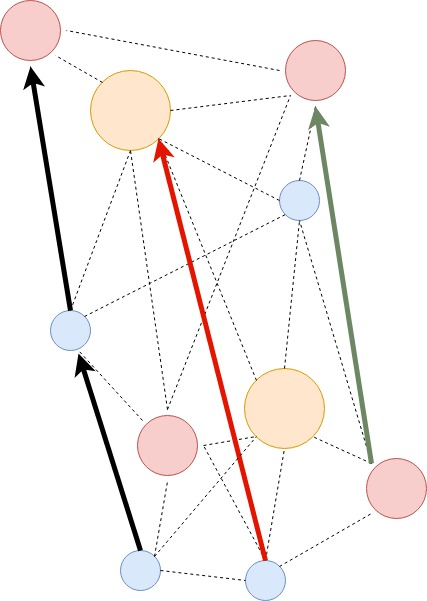
\includegraphics[scale=0.3]{fotos/shortestpath.jpg}}
\subfigure[konsolidierter Pfad]{\label{fig:b}
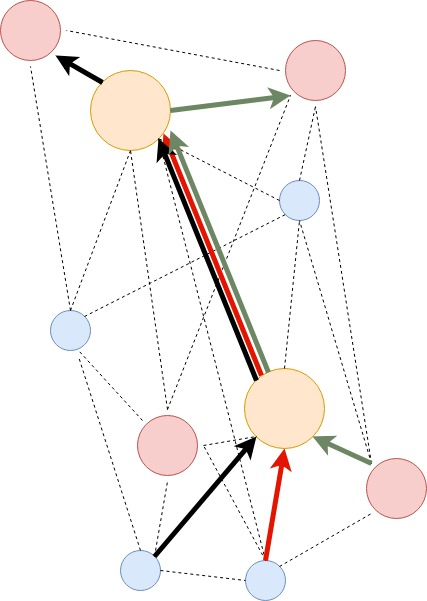
\includegraphics[scale=0.3]{fotos/cosolidated.jpg}}
\subfigure[gemischte Lösung]{\label{fig:c}
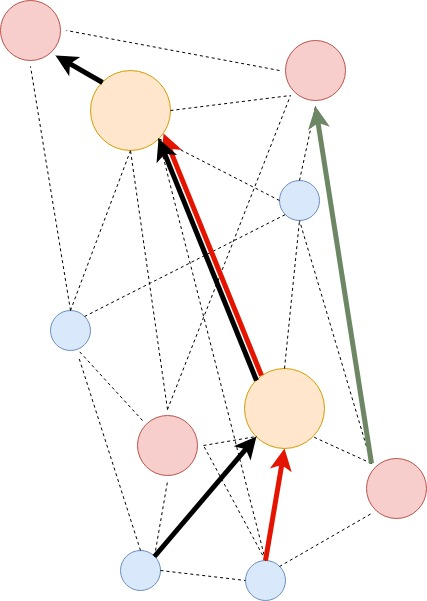
\includegraphics[scale=0.3]{fotos/mixedpath.jpg}}
\caption{Drei verschiedene Transportlösungen}
\end{figure}

\subsection{Problembeschreibung}
\label{sec:discription}
Die Modellierung eines Entscheidungsunterstützungssystems als ein Optimierungsproblem ist mit rechenbarem Ziel sowie Einschränkungen verbunden. Im folgenden Unterabschnitt wird die Nebenbedingungen sowie Zielfunktion des Modells konkret dargestellt.

\subsubsection{Nebenbedingungen}
In verschiedenen Szenarien (Probleminstanzen) gibt es verschiedene betriebliche Einschränkungen, deshalb soll der Anwender in der Lage sein, eine Kombination der Nebenbedingungen je nach Fragestellung auszuwählen.

\paragraph{Anzahl der Züge.}
Ein Zug besteht aus einigen Wagen, die mit einer bzw. mehreren Lokomotiven gezogen werden. Es ist zu beachten, dass die Merkmale der Züge im Konzept der Kanten integriert sind. Z.B. das maximal erlaubte Gewicht auf einer Blockkante bestimmt die Kapazität der Lokomotiven. Dementsprechend werden auf einer Kante mehrere Züge benötigt, falls das Gewicht der Sendungen auf der Kante diese Kapazität überschreitet.\\
Aus verschiedenen Gründen, wie z.B. begrenzte Gleislängen an den Rangierbahnhöfen oder Gleisabschnitte auf der Teilstrecke, haben die Züge eine andere Kapazität in Bezug auf die Länge. Ähnlich wie das Gewicht führt es ggf. zum Bedarf an mehreren Zügen.\\
Falls eine Kante von einer Sendung bzw. einigen Sendungen belegt wird, soll die Summe des Gewichts bzw. der Länge aller Sendungen kleiner gleich der möglichen Kapazität (Anzahl der Züge multipliziert mit dazugehöriger Kapazität) sein. Die Länge und das Gewicht konsolidierter Sendungen auf eine Kante bestimmen also, wie viele Züge hier benötigt werden.

\paragraph{Anzahl der Richtungsgleise.}
Die Fahrbahn der Schienenfahrzeuge wird als Gleis bezeichnet. Im Allgemeinen verbinden diese zwar zwei Bahnhöfe miteinander, aber jeder Bahnhof umfasst auch Richtungsgleise, in denen die Güterwagen zum Bilden neuer Züge rangiert werden. Nur eine gewisse Menge der Züge kann höchstens in einem Richtungsgleis der Anlage umgestellt werden. Falls die Anzahl der Züge in einer Richtung (die Züge mit gleichem Ziel) diese Kapazität überschreitet, werden mehrere Richtungsgleise belegt. Jeder Bahnhof hat jedoch eine begrenzte Anzahl der Richtungsgleise.

\paragraph{Anlage-Umstellkapazität.}
Abhängig von der Größe sowie technischer Ausstattungen jedes Bahnhofs ist  die Anzahl umstellbarer Wagen eingeschränkt. Die Rangierbahnhöfe verfügen über größere Umstellkapazität im Vergleich zu anderen Anlageklassen.

\paragraph{Leitwegbedingung}
die Restriktion bezieht sich auf eine strukturelle Beschränkung der Routenplanung, die mehrere Routen gleichzeitig betrifft. Die Leitwegbedingung erklärt, dass die Sendungen mit gleichem Ziel, die sich im Laufe ihrer Pfade durch das Verkehrsnetz in einem Knote treffen, auf dem verbleibendem Weg nicht mehr getrennt werden dürfen. Diese Restriktion ermöglicht praktischerweise die Komplexitätsreduktion bei der Steuerung der Sendungen. Die folgenden Bilder zeigen jeweils die erfüllte und die verletzte Leitwegbedingung.

\begin{figure}[h]
\subfigure[erfüllte Leitwegbedingung]{\label{fig:aa}
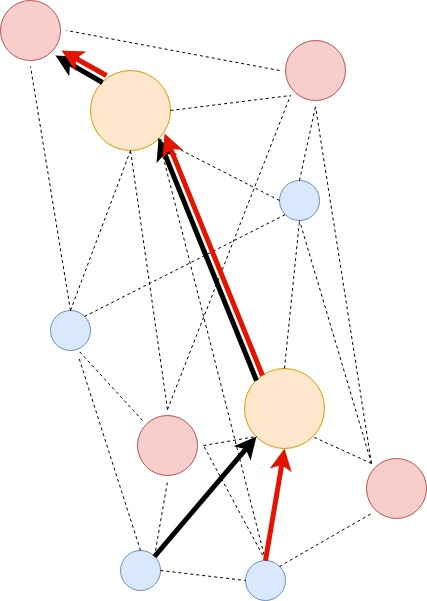
\includegraphics[scale=0.4]{fotos/uniqnuessstisfied.jpg}}
\subfigure[verletzte Leitwegbedingung]{\label{fig:bb}
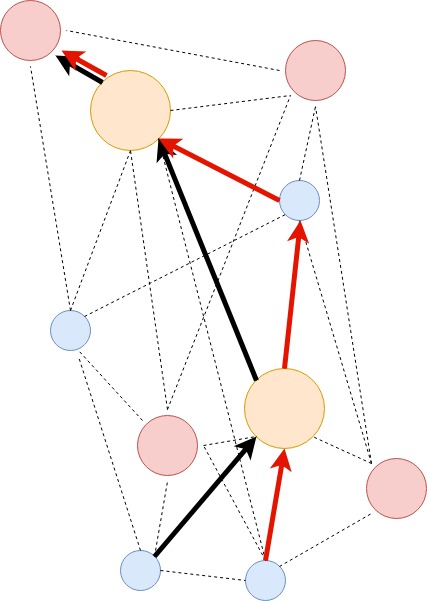
\includegraphics[scale=0.4]{fotos/uniqnuesviolated.jpg}}
\caption{Abbildung der Leitwegbedingung für Routen der zwei Sendungen mit gleichem Ziel}
\end{figure}

\paragraph{Transportzeit.}
Die Sendungen müssen ihr Ziel erreichen, und zwar rechtzeitig. Die Transportzeit bzw. der Zeitraum zwischen der Bereitstellung der Sendung im Quell-Knoten (spezifiziert durch den Parameter „Aufkommenszeitpunkt der Sendung“) und Ankunftszeit am Ziel soll das Zeitlimit, das durch den Parameter „Maximale Transportzeit“ jeder Sendung festgelegt ist, nicht überschreiten. Transportzeit der Sendung besteht aus verschiedenen Komponenten wie der echten Fahrtzeit, der Abfahrt-Bearbeitungszeit und Rangierzeit an den Zwischenbahnhöfen. Außerdem ist eine Wartezeit ggf. vorstellbar, falls eine Sendung zur Bündelung auf andere Sendungen, die noch nicht angekommen sind, in einer Zwischenanlage warten muss. Da die Sendungen Im zeitlichen Modell der Kanten mit konkreten Abfahrtzeiten zugeordnet werden, wird die Wartezeit auch implizit bestimmt.

\paragraph{Zielsetzung des Problems.}
wie schon in \hyperref[subsec:routenplan]{1.1.1} erklärt wurde, das Entscheidungsunterstützungssystem sollte den optimalen Routenplan herausfinden. Zur Optimierung des Routenplans werden die verursachten Kosten minimiert. Jede Lösung präsentiert also einen Routenplan mit der verursachten Kosten als Zielfunktionswert, und kann unter Berücksichtigung der genannten Restriktionen zulässig oder unzulässig sein. Im folgenden sind alle Kostenkomponenten nochmals zusammengefasst:

\begin{itemize}
    \item Zugkosten
    \item Umstellkosten
    \item Richtungsgleiskosten
    \item Anlagenfixkosten
    \item Wagenstundenkosten
    \item Transferzeitkosten
\end{itemize}

Es ist zu beachten, dass ein Routenplan die Zug- bzw. Gleisbelegung nicht explizit aufweist. Trotzdem sollen die Variablen zur Berechnung der Routenplan-Kosten generiert werden. Z.B. die Zugkosten einer Kante lässt sich mit der folgenden Formel rechnen.
\begin{equation*}
    \begin{aligned}
        & e_{ij}^t : \textit{Die Kante von i nach j mit der Abfahrtszeit t} \\
        & \textit{Zugkosten der Kante } e_{ij}^t  = \textit{Anzahl der Züge auf der } e_{ij}^t * \textit{Zugkosten der } e_{ij}^t
    \end{aligned}
\end{equation*}
Um die Anzahl der Züge auf der Kante $e_{ij}^t$ zu bestimmen, wird der Routenplan nach den Routen durchsucht, in denen die Kante $e_{ij}^t$ auftritt. Dementsprechend wird es durch die Summe des Gewichts bzw. der Länge der durchfahrenden Sendungen festgesetzt, wie viele Züge auf der Kante $e_{ij}^t$ benötigt werden. Ähnliches Verfahren wird zur Bestimmung der Knotenbelegung gefolgt, um die Anlagenfixkosten, die Umstellkosten und die Richtungsgleiskosten zu berechnen.\\

Da die Zielfunktion des Problems multikriteriellen Ziele (Kostenkomponenten) beinhaltet, und die Auswirkung jedes Ziels nach Auswertung der Anwender bei verschiedenen Szenarien steuerbar sein sollte, wird außerdem jeder Kostenkomponente eine Gewichtung zugeordnet, und die gewichtete Summe wird im Endeffekt als Zielfunktionswert genommen. Die Gewichtung einigt auch die Kosteneinheiten insbesondere für die Transferzeitkosten und Wagenstundenkosten.

\subsection{Aktueller Lösungsansatz}
\label{sec:current}
Der bestehende Lösungsansatz basiert auf der Dissertation von Dr. Henning \cite{homfeld2012consolidating}. Die von Homfeld bearbeitete Problematik beinhaltet zwar keine regulären Abfahrtzeiten, aber eine zusätzliche Nebenbedingung mehr die sog. „Hierarchie Bedingung“. Diese Restriktion beschränkt den Routenplan je nach den auf Bahnhof-Klassen basierenden Vorschriften. Da die Anlagen sich in Größe und technische Ausstattungunterscheiden, sind bei der Deutschen Bahn die Bahnhöfe in vier Klassen eingestuft: Ebene-0 Rangierbahnhöfe, Ebene-1 Knotenbahnhöfe, Ebene-2 Mittelbahnhöfe und Ebene-3 Anlieferungsbahnhöfe angeordnet.\\

Dementsprechend gibt es zurzeit zwei Ansätze (heuristisch und exakt) für jede Problemstellung (Hierarchie-Modell und Zeit expandiertes Modell). Im folgenden werden die einzelnen Arbeitsschritte zusammengefasst erklärt.

\subsubsection{Graph-Transformation}
Bezüglich der vom Anwender ausgewählten Problemstellung wird zunächst der Verkehrsgraph des Szenarios transformiert. Sind also reguläre Abfahrtzeiten relevant, wird der Graph zeitlich expandiert. Ist aber umgekehrt die Hierarchie-Bedingung wichtig, wird der Verkehrsgraph so transformiert, dass die Hierarchie-Bedingung erfüllt wird.

\paragraph{Zeitliche Expansion.}
Wie schon erwähnt wurde, hat jede Kante täglich reguläre Abfahrtzeiten. Der Graph des Verkehrsnetzwerks des jeweiligen Szenarios wird daher zunächst zeitlich expandiert. Durch die Expansion werden die Kanten und Knoten zeitlich angepasst. Bild 3 zeigt, wie beispielweise die Anlage $A$ und $B$ sowie Kante $AB$ mit täglich 4 Abfahrtzeiten nach der Zeitexpansion darzustellen sind.

\begin{figure}[ht]
\centering
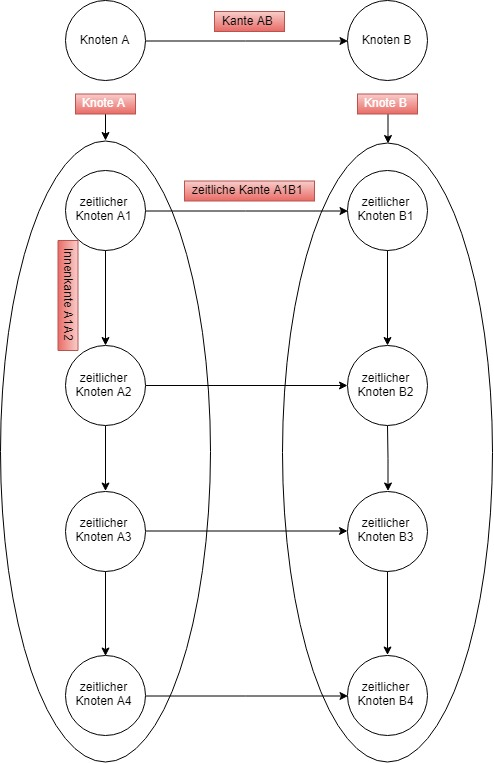
\includegraphics[scale=0.3]{fotos/timeexpansion.jpg}
\caption{Darstellung der Zeitexpansion}
\end{figure}

Da die zeitlichen Knoten $A^{t_i}$ und $B^{t_j}$ sowie die zeitlichen Kanten $AB^{t_i} $ ($t_i$ bezeichnet die Abfahrtzeit der Kante) nur die Zeitkomponenten des ersten Tages abbilden, werden die zeitliche Knoten und Kanten in den folgenden Tagen des Planungshorizonts ausgerollt. Die maximale Transportzeit in der Menge der Sendungen wird als den Planungshorizont angenommen. Die räumliche Knoten $A$ und $B$ sowie die Kante $AB$ bekommen also nach der Expansion die Zeitkomponenten $A^{t_i, m. Tag}$ , $B^{t_j, m. Tag}$ und $AB^{t_i, m. Tag}$. $AB^{t_i, m. Tag}$ bezeichnet also die Kante $AB$, die am Tag $m$ um $t_i$ abfährt.\\

falls es an der A und B Knoten noch weiteren Abfahrten gäbe, würden dementsprechend mehrere Zeitliche Knoten und Kanten erzeugt.

\subsubsection{Heuristischer Lösungsansatz}
Der heuristische Ansatz vorgeschlagen von \cite{homfeld2012consolidating} und basierend auf dem Fluss-Model „Rip-up and Reroute“ versucht, erstmals eine Initiallösung zu erzeugen. Danach werden die Routen einiger Sendungen vom Initial-Routenplan ausgenommen und wieder geroutet. Der vorherige Schritt wird iterativ fortgesetzt, sobald das Terminierungskriterium getroffen wird.

\subsubsection{Mathematische Modellierung}
Schließlich wird ein MIP-Model mit den verschiedenen Entscheidungsvariablen er-stellt. Die drei wichtigsten Entscheidungsvariablen sind die Flussvariablen sowie Zugvariablen und Richtungsgleis-Variablen. Zur Modellierung der Leitwegbedingung wird eine zusätzliche Entscheidungsvariable, die sog. „Baumvariable“ hinzugefügt. Sind ungeroutete Sendungen erlaubt, wird dazu jeweils eine Entscheidungsvariable definiert.\\
Anhand eines MIP-Solvers (Gurobi oder Cplex) wird das Model schließlich gelöst. Die beste heuristische Lösung kann dem MIP-Solver als Initiallösung eingegeben werden.\\
Es wurde wie beschrieben jeder Kostenkomponente eine Gewichtung zugeordnet. Damit kann man die Auswirkung der Kostenbestandteile jeweils beliebig verstärken oder sogar komplett ausschalten, falls die Gewichtung gleich null gesetzt wird. Das Problem bei den unterschiedlichen Kosteneinheiten wurde mithilfe eines Faktors behoben, der Zeit-Einheit in Geld-Einheit umwandelt.


\section{Zielsetzung dieser Arbeit}
\label{sec:Ziel}
Die Zeitexpansion vergrößert rasant den räumlichen Verkehrsgraphen, und erzeugt viele zeitlichen Knoten und Kanten, worauf aber der jetzige heuristische Lösungsansatz \emph{(Rip-up and Reroute)} nicht gut reagiert. Sogar mit langer Rechenzeit und tausenden Iterationen fällt normalerweise eine relativ große Lücke zwischen dem besten gefundenen Zielfunktionswert von R\&R und dem MIP-Solver als angewandter exakter Lösungsansatz auf.\\
Nach der Besprechung mit den Fachexperten der Deutschen Bahn sowie dem Lehrstuhl, dem diese Arbeit vorgelegt wird, also Wirtschaftsinformatik insb. Operations Research der Universität Paderborn, wurde die Implementierung und durch diese Abschlussarbeit Dokumentation eines pfad-basierten heuristischen Lösungsansatzes für die beschriebene Problemstellung als Ziel ausgewählt.


%\section{Vorgehensweise}
